%----------------------------------------------------------------
%
%  File    :  thesis.tex
%
%  Authors :  Keith Andrews, IICM, TU Graz, Austria
%             Manuel Koschuch, FH Campus Wien, Austria
% 
%  Created :  22 Feb 96
% 
%  Changed :  24 March 2009
% 
%----------------------------------------------------------------

% Please send any questions, comments, remarks or complaints to
% manuel.koschuch@fh-campuswien.ac.at


% --- General Setup ---------------------------------------------

%\documentclass[14pt,a4paper,oneside]{extbook} %war 12pt, wieder ändern!!!
\documentclass[12pt,a4paper,oneside]{article} %11original
%\usepackage{times}

%\renewcommand{\rmdefault}{phv} % Arial
%\renewcommand{\sfdefault}{phv} % Arial

\usepackage[utf8]{inputenc}   % so can use Umlaut chars  
\usepackage[T1]{fontenc}
\usepackage[bf,sf]{subfigure}
\renewcommand{\subfigtopskip}{0mm}
\renewcommand{\subfigcapmargin}{0mm}

\usepackage[english]{babel}         % load babel *before* natbi
%\usepackage[austrian]  % load babel *before* natbi
%\usepackage[square]{natbib}                  % citations
\usepackage{enumitem}
\usepackage{url}

\usepackage{float}

\usepackage{latexsym}

\usepackage{color}

\usepackage{ifpdf} % detect outputstyle

\usepackage{geometry} % define pagesize in more detail

\usepackage{fancyhdr} % nicer headers and footers
\usepackage{eurosym}
\usepackage{url}
\usepackage{colortbl} %define colored backgrounds for tables
\usepackage{booktabs}
\usepackage{tabularx}
\usepackage{fancyhdr}
\usepackage{multirow}
\ifpdf
  \usepackage[pdftex]{graphicx}
  \DeclareGraphicsExtensions{.pdf,.jpg,.png}
  \pdfcompresslevel=9
  \pdfpageheight=297mm
  \pdfpagewidth=210mm
\usepackage{fixltx2e}
  \usepackage[         % hyperref should be last package loaded
    pdftex,
    bookmarks,
    bookmarksnumbered,
    linktocpage,
    pagebackref,
    pdfview={Fit},
    pdfstartview={Fit},
    pdfpagemode=UseOutlines,                 % open bookmarks in Acrobat
  ]{hyperref}
  \usepackage{bookmark}
\else                      % latex
  \usepackage{graphicx}
\usepackage[T1]{fontenc} 
{\fontfamily{Schriftart}\selectfont Text}
\usepackage{color}
  \DeclareGraphicsExtensions{.ps}
\fi
 \usepackage{rotating}
\newcommand\tabrotate[1]{\begin{turn}{90}\rlap{#1}\small\end{turn}}

\geometry{a4paper,left=24mm,right=24mm, top=30mm, bottom=30mm} %hier waren original 25,35,30,30

\setlength{\parskip}{3pt plus 1pt minus 0pt}       % vert. space before a paragraph

\setcounter{tocdepth}{1}        % lowest section level entered in ToC
\setcounter{secnumdepth}{2}     % lowest section level still numbered




% --- Start of Document ----------------------------------------


\begin{document}


\begin{picture}(50,50)
\put(-70,40){\hbox{\includegraphics{images/header.png}}}
\end{picture}

\vspace*{-5.8cm}

\begin{center}

\vspace{9.9cm}

\hspace*{-1.0cm} {\LARGE \textbf{Design document\\}}
\vspace{0.2cm}
\hspace*{-1.0cm}  \\

\vspace{0.65cm}


\vspace{0.65cm}
\vspace{3 cm}
\hspace*{-1.0cm} { \textbf{Group Nr. 3\\}}
\vspace{1cm}

\hspace*{-1.0cm} { \textbf{ Timur Ali Basnakajev\\}}
\hspace*{-1.0cm} { \textbf{ Tobias König\\}}
\hspace*{-1.0cm} { \textbf{ Jessica Marban\\}}
\hspace*{-1.0cm} { \textbf{ Patrick Neumann\\}}
\vspace{0.2cm}
\hspace*{-1.0cm}  \\

\end{center}              % Title Page
\tableofcontents

%--- Include your chapters here ----------

\include{projectdescription} 
\section{Software architecture and design}
\label{chapter2}

\subsection{Software modules}

\subsubsection{Safety related modules}
\begin{enumerate}
    \item \textbf{CO2 Sensor Measurement and Validation Module (Arduino):} \\ 
        \textbf{Description:} This module reads CO2 concentration levels using the MH-Z19 sensor and validates the readings to ensure they fall within a typical range. If a reading is outside the acceptable range, the value is marked as invalid and appropriate actions are taken. Valid CO2 values are sent to the Raspberry Pi for further processing. \\ 
        \textbf{Functions:}
        \begin{itemize}
            \item Measure CO2 concentration as an analog value using the MH-Z19 sensor.
            \item Validate the analog reading to ensure it falls within a typical range.
            \item Mark and handle invalid values (e.g., send an error message or retry reading).
            \item Send validated CO2 concentration values to the Raspberry Pi via serial communication.
        \end{itemize}
        \textbf{Data:} Raw sensor data, validated CO2 concentration values (ppm). \\ 
        \textbf{Requirements:} \ref{req.2},  \ref{req.2.1}, \ref{req.2.2}\\

    \item \textbf{Window Control Module (Raspberry Pi):} \\ 
        \textbf{Description:} This module receives validated CO2 values from the Arduino and controls the electric motor to open or close the window based on the CO2 levels. It ensures safe operation by detecting any obstacles during movement. \\ 
        \textbf{Functions:}
        \begin{itemize}
            \item Receive validated CO2 concentration values from the Arduino.
            \item Open/close the window using the stepper motor if CO2 levels exceed or drop below predefined thresholds.
            \item Monitor motor movement and detect deviations during window operation.
            \item Stop motor and trigger an error state if obstacles are detected.
            \item Report errors through email and LED indicators.
        \end{itemize}
        \textbf{Data:} Stepper motor position, window state, validated CO2 data. \\ 
        \textbf{Requirements:} \ref{req.3},  \ref{req.3.1}, \ref{req.3.2}, \ref{req.3.3} \\
        \newpage
    \item \textbf{Fan Control Module (Raspberry Pi):} \\ 
        \textbf{Description:} This module controls the fan based on the CO2 levels received from the Arduino. It turns the fan on when CO2 levels are high and turns it off when levels normalize. \\ 
        \textbf{Functions:}
        \begin{itemize}
            \item Turn on the fan when the CO2 level surpasses a certain threshold.
            \item Turn off the fan when CO2 levels fall below the desired range.
        \end{itemize}
        \textbf{Data:} CO2 concentration values, fan state. \\ 
        \textbf{Requirements:} Related to system operation based on CO2 levels.
\end{enumerate}

\subsubsection{Security related modules}
\begin{enumerate}
    \item \textbf{Communication Encryption Module:} \\ 
        \textbf{Description:} This module ensures secure data transmission between the Raspberry Pi and Arduino to prevent unauthorized access and tampering. It requires both the Raspberry Pi and Arduino to handle encryption and decryption of messages. \\ 
        \textbf{Functions:}
        \begin{itemize}
            \item On the Raspberry Pi, encrypt data using the `cryptography` library before sending it to the Arduino.
            \item On the Arduino, use an AES-compatible library (e.g., Arduino Cryptography Library) to decrypt the received data.
            \item Ensure both devices securely share the encryption key for symmetric encryption.
        \end{itemize}
        \textbf{Data:} Encrypted communication data. \\ 
        \textbf{Requirements:} \ref{sreq.1} \\

    \item \textbf{System Hardening Module (Raspberry Pi):} \\ 
        \textbf{Description:} This module focuses on securing the Raspberry Pi against cyber threats. It ensures that the Raspberry Pi is protected from unauthorized access. \\ 
        \textbf{Functions:}
        \begin{itemize}
            \item Manage user authentication and access control.
            \item Implement firewall rules to restrict network access.
            \item Monitor and log suspicious activity.
        \end{itemize}
        \textbf{Data:} Security logs, access control records. \\ 
        \textbf{Requirements:} \ref{sreq.2} \\
\end{enumerate}

\subsubsection{Modules with no influence on Safety and Security}
\begin{enumerate}
    \item \textbf{System Monitoring Module (Raspberry Pi):} \\ 
        \textbf{Description:} This module handles general system diagnostics like checking CPU temperature and memory usage. It ensures that non-critical parameters are monitored for optimal system performance. \\ 
        \textbf{Functions:}
        \begin{itemize}
            \item Monitor system health, such as CPU temperature and memory usage.
            \item Provide status updates about system performance.
            \item Log non-critical warnings for maintenance purposes.
        \end{itemize}
        \textbf{Data:} System diagnostics logs, performance metrics. \\ 
        \textbf{Requirements:} \ref{qreq.1}.
\end{enumerate}

\subsection{Libraries}
The following libraries are used to interface with hardware components and to implement the functionality described above:
\begin{itemize}
    \item \textbf{MH-Z19 Library:} 
        \begin{itemize}
            \item **Arduino**: `MHZ19uart` or `SoftwareSerial` - to read CO2 data via UART from the MH-Z19 sensor and convert it into ppm values.
            \item **Raspberry Pi**: `pyserial` - for reading sensor data sent by the Arduino.
        \end{itemize}
    \item \textbf{Stepper Motor Control Library:} 
        \begin{itemize}
            \item **Raspberry Pi**: `RPi.GPIO` or `gpiozero` - to control the stepper motor for window movement.
        \end{itemize}
    \item \textbf{Email Notification Library:} `smtplib` (Python) - for sending email alerts directly from the Raspberry Pi when error states are detected.
    \item \textbf{Encryption Libraries:}
        \begin{itemize}
            \item **Raspberry Pi**: `cryptography` (Python) - for encrypting communication before sending it to the Arduino.
            \item **Arduino**: `Arduino Cryptography Library` - for decrypting the received encrypted messages.
        \end{itemize}
    \item \textbf{Firewall Configuration Tools:} `ufw` (Linux tool) - for setting up and managing firewall rules on the Raspberry Pi.
\end{itemize}

\subsection{Interrupts}
\textbf{Definition of priorities:}
\begin{itemize}
    \item \textbf{Priority 1:} Communication failure detection interrupt between the Raspberry Pi and Arduino. This ensures immediate action if data transfer fails.
    \item \textbf{Priority 2:} Window control interrupts for obstacle detection during motor operation to prevent damage.
    \item \textbf{Priority 3:} CO2 sensor data validation on the Arduino to ensure accurate measurement.
\end{itemize}

\subsection{Pinout}
\begin{itemize}
    \item \textbf{CO2 Sensor (MH-Z19 - Arduino):} Connected via UART for analog data reading.
    \item \textbf{Window Motor Control (Raspberry Pi):} Connected to GPIO pins for controlling the motor.
    \item \textbf{Fan Control (Raspberry Pi):} Connected to GPIO pins for fan activation.
    \item \textbf{Error Indicators (Raspberry Pi):} LED connected to GPIO pins for status indication.
\end{itemize}

\section{Program flowchart}
\label{chapter3}


\begin{figure}[h]
	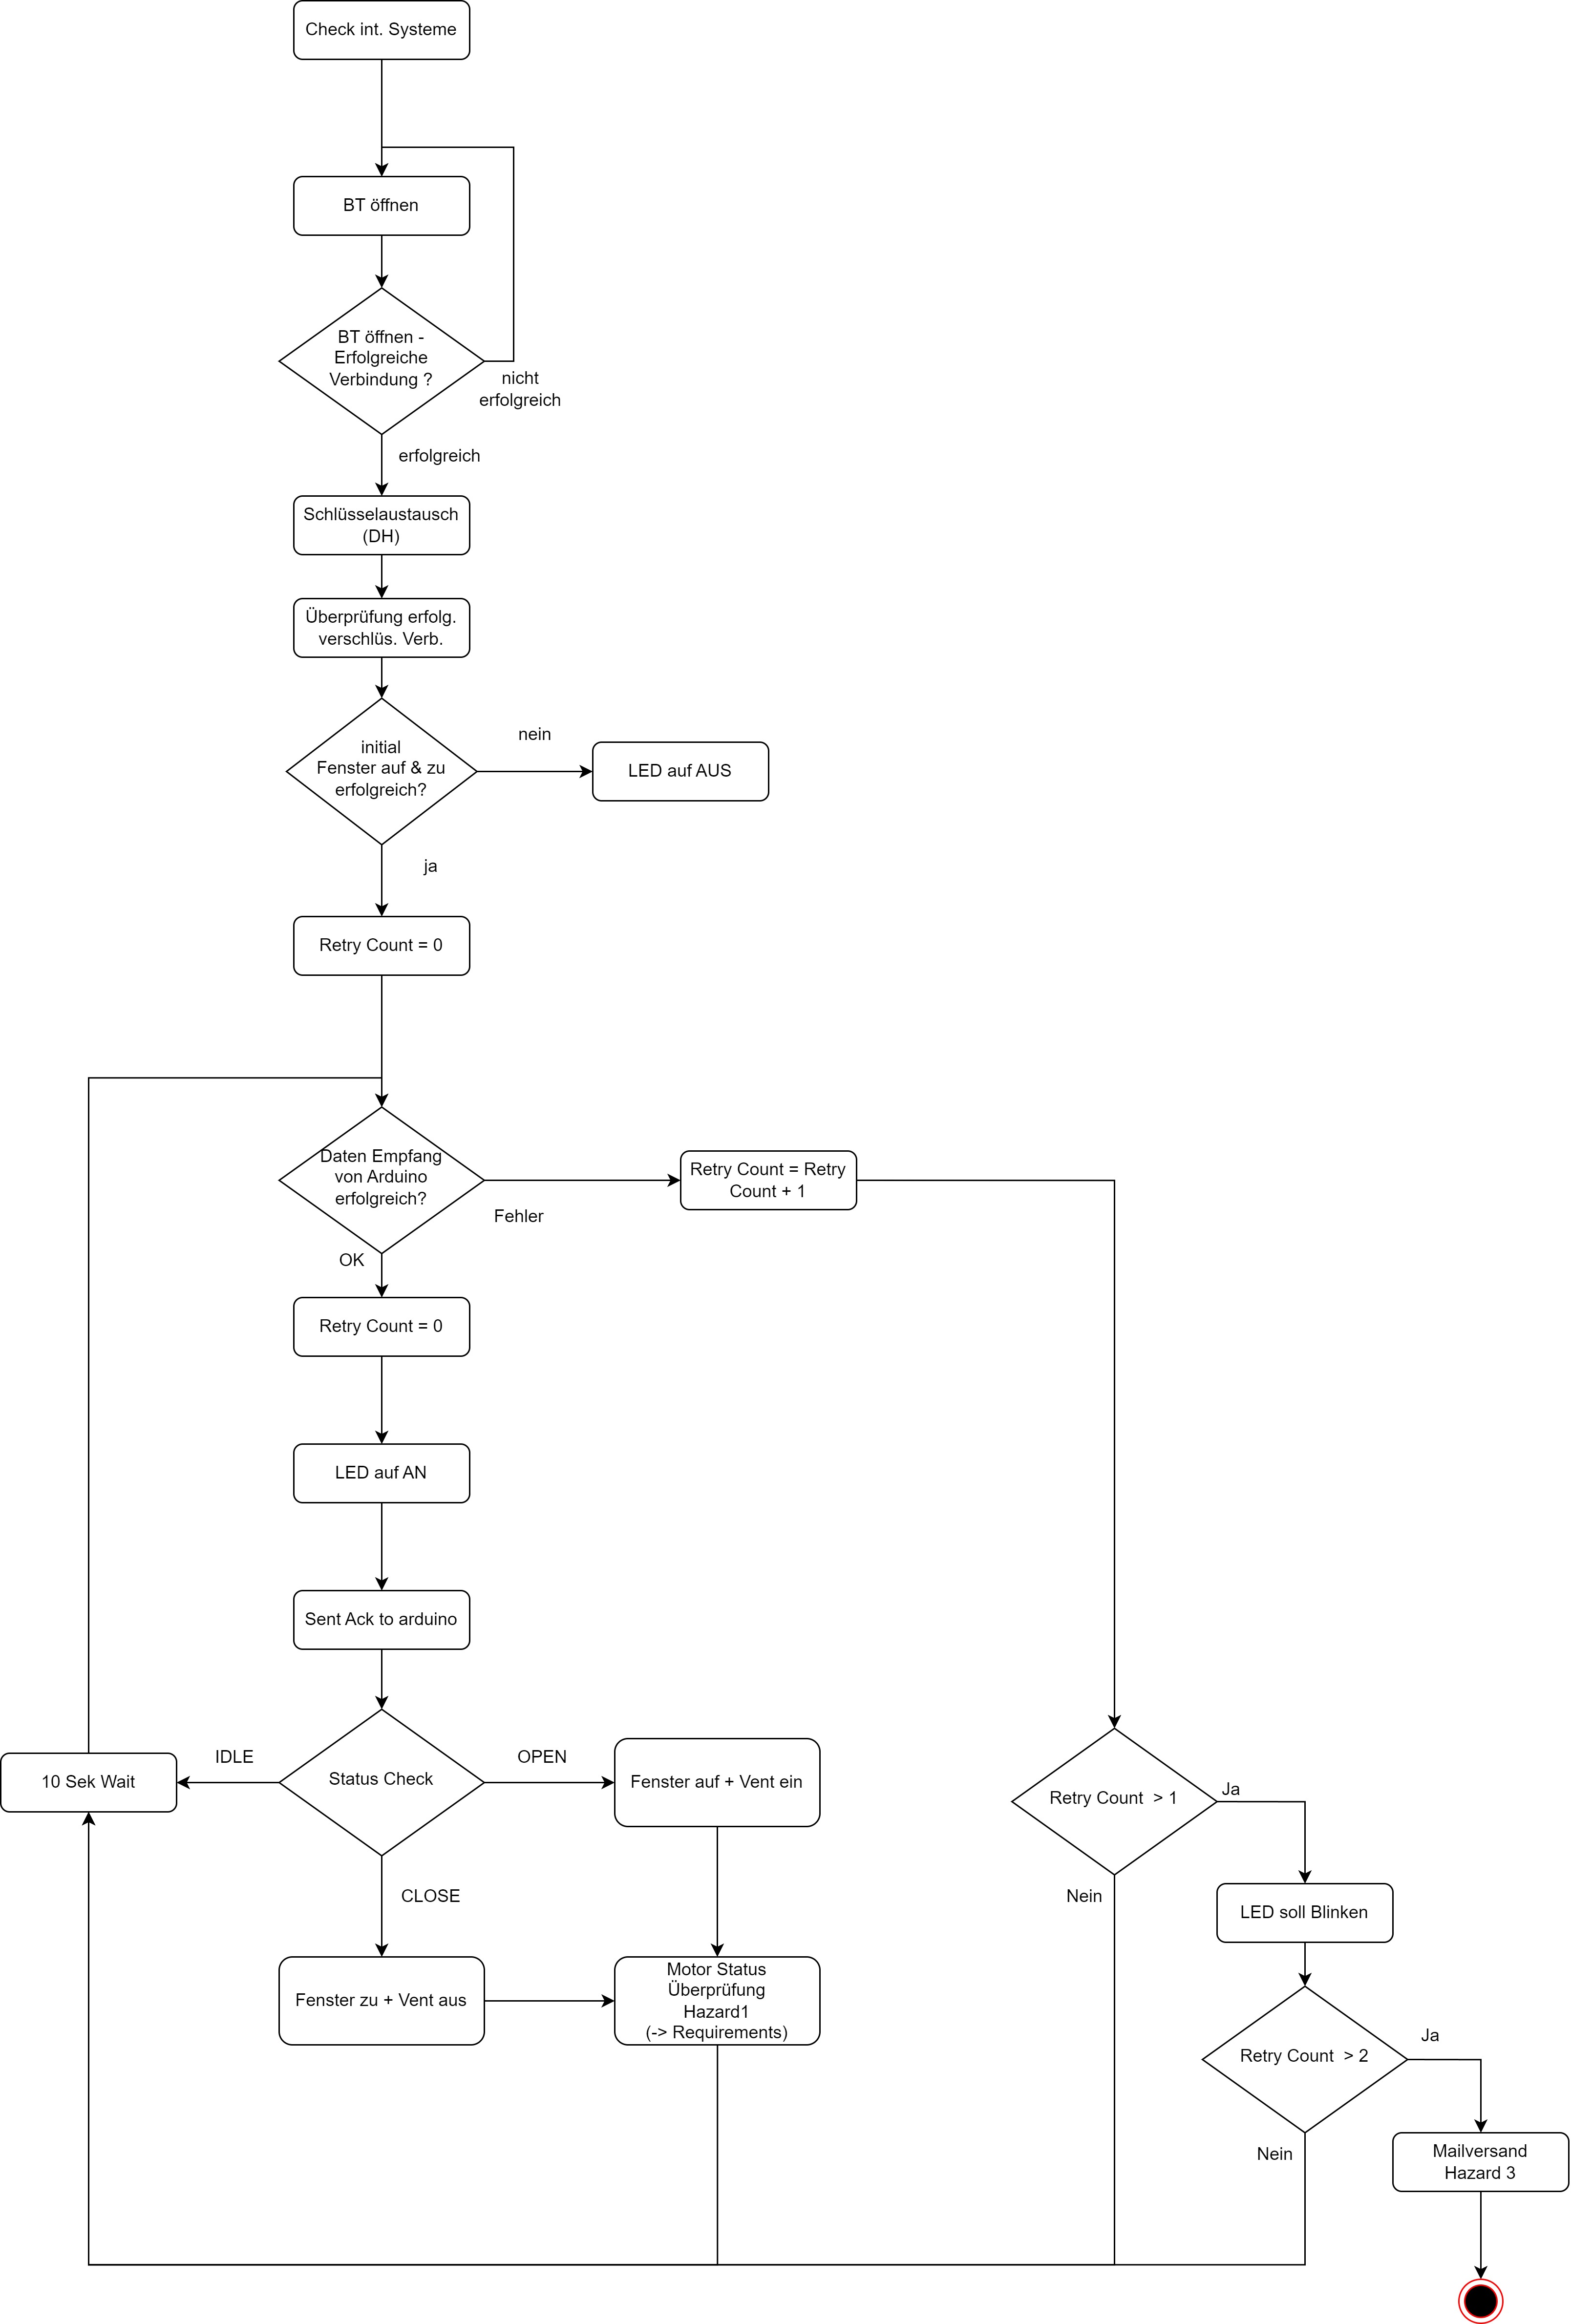
\includegraphics[height=170mm,left]{images/ablaufdiag_pi.jpg}
	\centering
	\caption{Rasperry PI}
	\label{fig:system}
\end{figure}

\begin{figure}[h]
	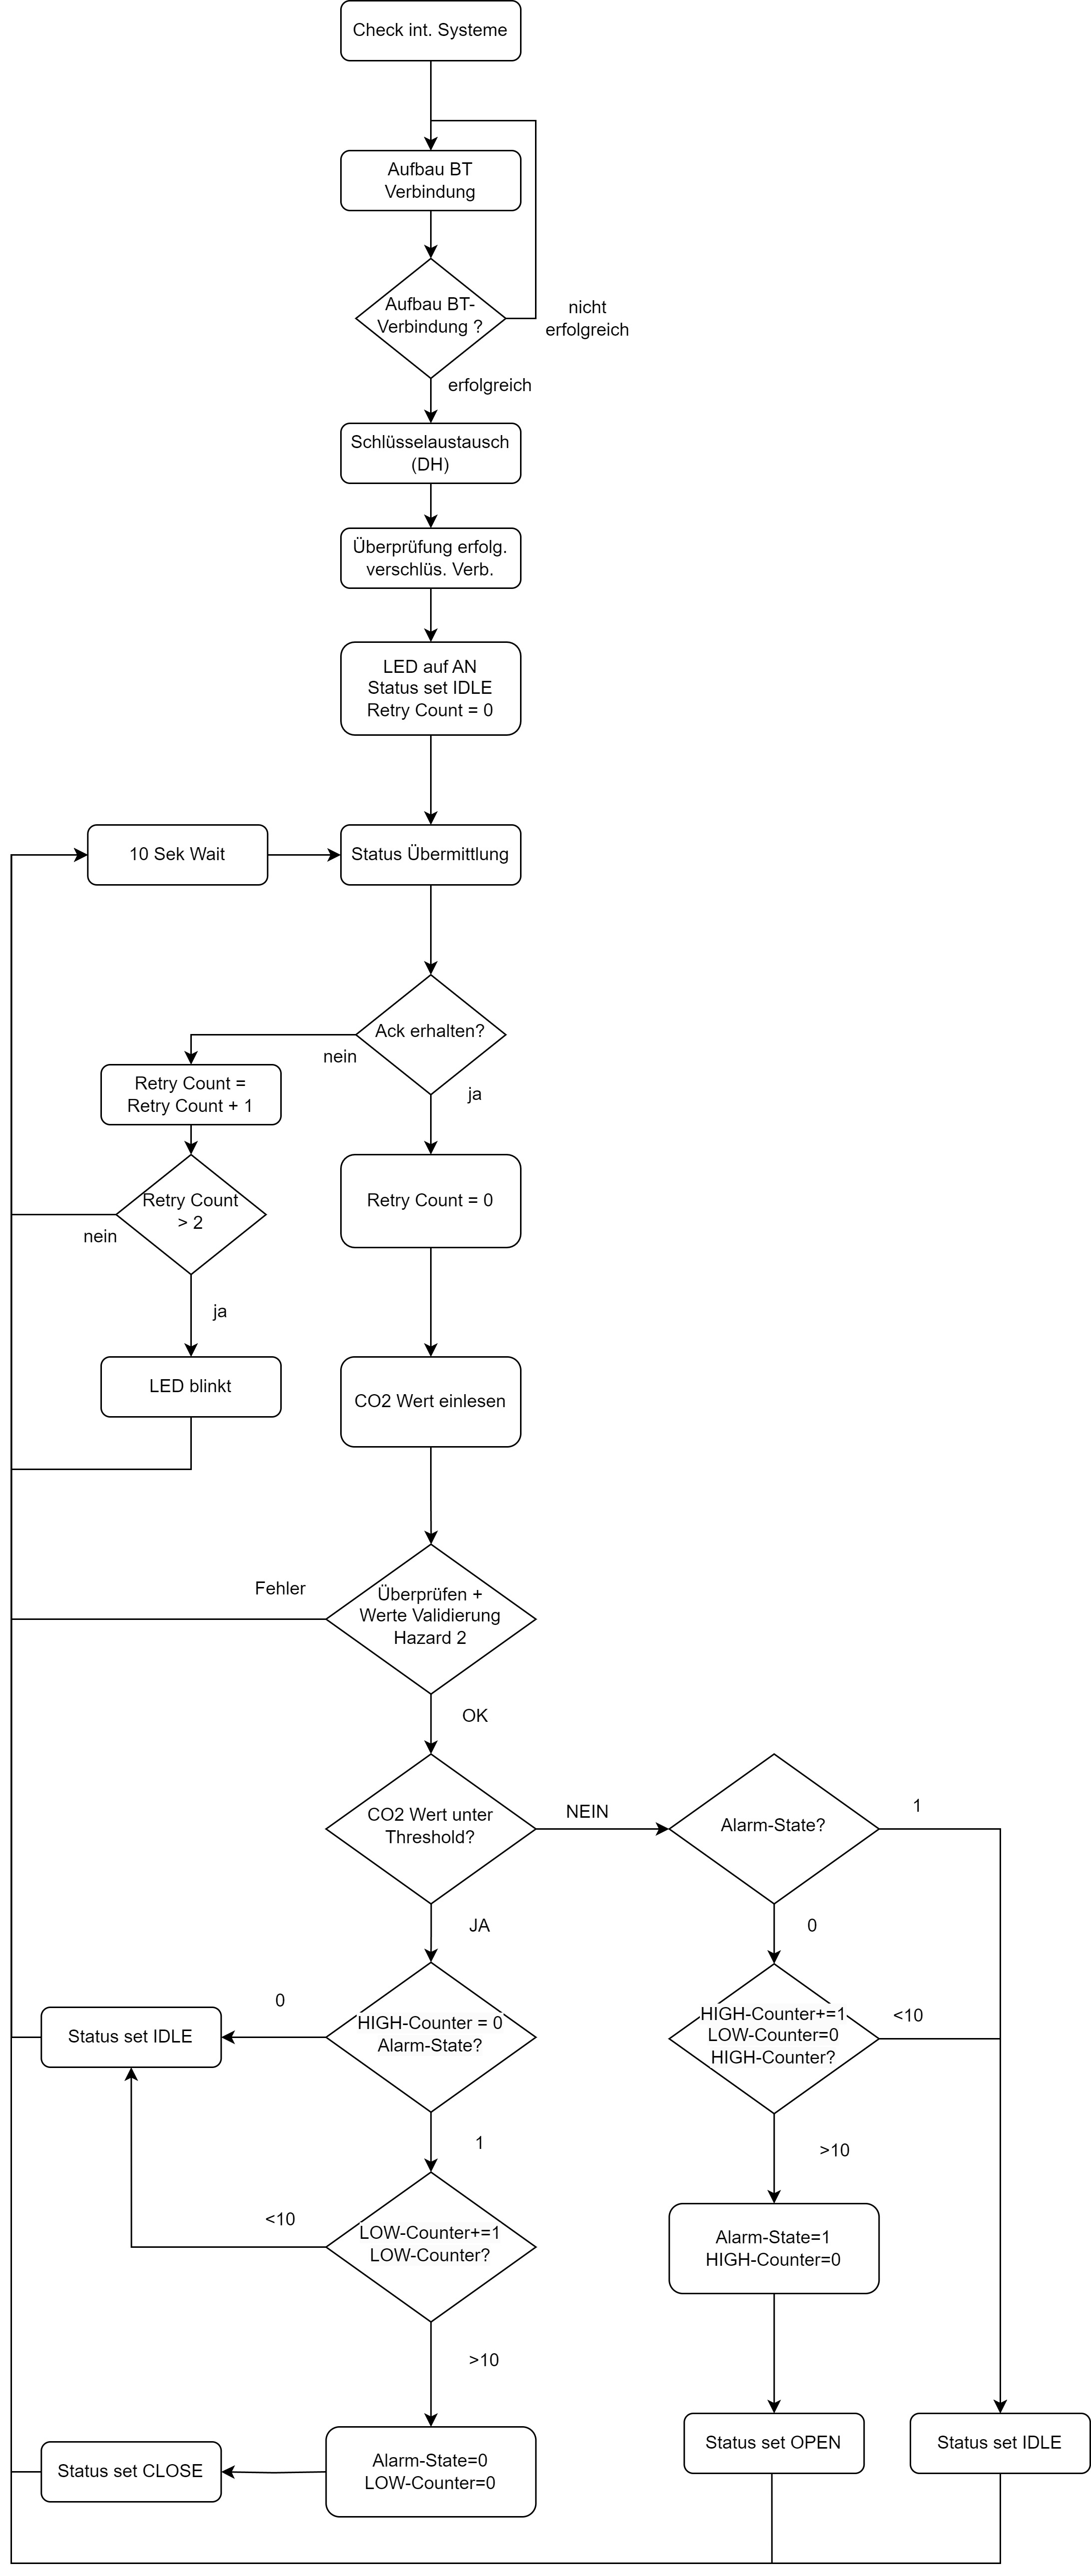
\includegraphics[height=190mm,left]{images/ablaufdiag_adriuno.jpg}
	\centering
	\caption{Arduino}
	\label{fig:system}
\end{figure}
\section{Hazard identification}
\label{chapter4}

\subsection{Identified hazards and countermeasures}


	\begin{enumerate}
		\item Hazard 1: \\
			Requirement see \ref{req.1.1} \\
		\item Hazard 2:
		\item Hazard 3:
	\end{enumerate}
	
\subsection{Identified hazards without countermeasures }

	\begin{enumerate}
		\item Hazard 1: \\
		\item Hazard 2:
		\item Hazard 3:
	\end{enumerate} 
\section{Threat identification}
\label{chapter3}

\subsection{Identified threats and countermeasures}

	\begin{enumerate}
		\item  \textbf{Threat 1:}
            An attacker can make a log lose or confuse data. \\ \\         
             \textbf{Mitigation:}
            There must be logs with timestamps.
		\item \textbf{Threat 2}:
            An attacker can alter the data that is sent back and forth.\\ \\
            \textbf{Mitigation:}
            Each message between the Arduino and Raspberry Pi must be accompanied by an HMAC.
		\item \textbf{Threat 3}:
            An Attacker carry out a DoS attack on the Raspberry Pi.\\ \\
            \textbf{Mitigation:}
            The Raspberry Pi must accept no more than 1 message every 9 seconds from the Arduino to prevent flooding attacks.	\end{enumerate}
	
\subsection{Identified threats without countermeasures}

	\begin{enumerate}
		\item \textbf{Threat 1:} 
            An attacker can force data through different validation paths which give different results. 
		\item \textbf{Threat 2:}
            An attacker can provide or control state information.
		\item \textbf{Threat 3:}
            An attacker can replay data without detection.            
	\end{enumerate} 
\section{Requirements}
\label{chapter4}



\subsection{Safety related requirements}

	\begin{enumerate}[label*=\arabic*.]
		\item \label{req.1}  Requirement: Connection Handling \\
		\begin{enumerate}[label*=\arabic*.]
			\item \label{req.1.1}  Requirement:  \\
			If an error occurs during program start at the Arduino, this must be indicated by an LED (LED OFF)\\ 
			\item \label{req.1.2} Requirement:   \\
			If no error occurs during program start at the Arduino, this must be indicated by an LED (LED ON)\\ 
			\item \label{req.1.3} Requirement:   \\
			If no error occurs during program start at the Raspberry Pi, this must be indicated by an LED (LED ON)\\    
			\item \label{req.1.4} Requirement:   \\
			If an error occurs during program start at the Raspberry Pi, this must be indicated by an LED (LED OFF)\\    
			\item \label{req.1.5} Requirement:   \\
			If the Arduino stops communicating with Raspberry Pi, the Raspberry Pi must send an email to the system administrator after connection-retries are unsuccessful for 30 seconds.\\    
   			\item \label{req.1.6} Requirement:   \\
            Connection-retries must be sent every 10 seconds.\\
			\item \label{req.1.7} Requirement:   \\
            When the connection is established initially and the devices are communicating, the window must be successfully opened and closed once as a mechanical functionality test.\\
		\end{enumerate}
		\item \label{req.2}  Requirement:  Invalid Value Handling\\
  	\begin{enumerate}[label*=\arabic*.]
			\item \label{req.2.1}  Requirement:  \\
			Every measured value of the CO2 sensor must be checked for their validity by the Arduino.\\ 
   		\item \label{req.2.2}  Requirement:  \\
			If the measured value differentiates more than 50 ppm from the average of the 5 previous values, the value is marked as invalid.\\
   		\item \label{req.2.3}  Requirement:  \\
			If the sensor value is marked as invalid, the value must be dropped.\\
	  \end{enumerate}
		\item \label{req.3}  Requirement:    Communication between devices  \\
  	\begin{enumerate}[label*=\arabic*.]
			\item \label{req.3.1}  Requirement:  \\
			  For every message sent between the Raspberry Pi and the Arduino, the receiving device must send an acknowledgement-message to the original sender.\\
   		\item \label{req.3.2}  Requirement:  \\
			If the Arduino doesn't get an acknowledgement-message for one of his status messages, it must resend this message.\\
   		\item \label{req.3.3}  Requirement:  \\
			Not acknowledged resend-messages must be sent every 10 seconds.\\
   		\item \label{req.3.4}  Requirement:  \\
			If 1 following resend-messages are not acknowledged, an LED on the Arduino must start blinking.\\ 
	  \end{enumerate}  
        \item \label{req.4}  Requirement: Operating the window \\
  	\begin{enumerate}[label*=\arabic*.]
			\item \label{req.4.1}  Requirement:  \\
            It must be checked whether the window has been opened or closed sufficiently, by comparing the measured end-position of the stepper motor with the value of a fully opened or closed window\\  
			\item \label{req.4.2}  Requirement:  \\
            If the measured end-position of the stepper motor deviates by 1 cm from the value of a fully opened window when opening, the motor must stop immediately and go back into its starting position.\\   
			\item \label{req.4.3}  Requirement:  \\
			If the measured end-position of the stepper motor deviates by 1 cm from the value of a fully closed window when closing, the motor must stop immediately and go back into its starting position.\\  
			\item \label{req.4.4}  Requirement:  \\
		      After the stepper motor has to reset to his starting position when opening or closing the window, it must retry the opening or closing process a second time after 10 seconds.\\  
			\item \label{req.4.5}  Requirement:  \\
			If the opening or closing process of the windows doesn't work a second time an error has to be displayed by the Raspberry Pi through an blinking LED.\\  
	  \end{enumerate}         
	\end{enumerate}


 

\subsection{Security related requirements}
    \begin{enumerate}[label*=\arabic*.]
        \item \label{sreq.1} Spoofing Requirement:  \\
        Both devices (Arduino and Raspberry Pi) must share a pre-shared key (PSK), which is used for authentication and integrity verification. For each communication, the sender computes an HMAC using the message and the secret key. The receiver uses the same key to validate the HMAC. \\ 
        To exchange the key, both devices must use the Diffie-Hellman key exchange.\\
        Both devices must have a unique device ID that is checked to ensure that only authenticated devices are allowed to communicate.\\
        \item \label{sreq.2} Tampering Requirement:  \\
        Each message between the Arduino and Raspberry Pi must be accompanied by an HMAC to verify whether the message has been altered during transmission. \\ 
        Unauthorized physical access of the Raspberry Pi or Arduino should be prevented.\\
        \item \label{sreq.3} Repudiation Requirement:  \\
        Each sent and received packet must be logged with timestamps on the Arduino and the Raspberry Pi. \\ 
        Critical actions, such as opening and closing the windows, must also be logged.\\
        \item \label{sreq.4} Information Disclosure Requirement:  \\
        The communication over the Bluetooth connection between the Raspberry Pi and the arduino must be encrypted via AES-CBC-128. \\
        The successful encryption must be verified. This could be done by sending an encrypted default string with the data for the devices to verify the encryption.\\
        \item \label{sreq.5} Denial of Service Requirement:  \\
        The Raspberry Pi must accept no more than 1 message every 9 seconds from the Arduino to prevent flooding attacks. \\
        The Arduino must only wait for 1 acknowledgement message after sending a data message to the Raspberry Pi.\\
        The Arduino must ignore all other received acknowledgement messages.\\
        \item \label{sreq.2} Elevation of Privilege Requirement:  \\
        There is a minimum length for the password of 12 characters. This guarantees a strong password which will make it hard for attackers to take over control of the administrators account.\\ 
    \end{enumerate}         



\subsection{Requirements with no influence on Safety and Security}
    \begin{enumerate}[label*=\arabic*.]
        \item \label{qreq.1}  Requirement:  \\
        The Raspberry Pi must be waiting for the Arduino to establish a Bluetooth Connection. \\ 
        \item \label{qreq.2}  Requirement:  \\
        The Adruino must initiate a Bluetooth Connection to the corresponding Raspberry Pi. \\ 
        \item \label{qreq.3}  Requirement:  \\
        If Bluetooth communication fails (no acknowledgment received), the Raspberry Pi must attempt to reconnect up to 3 times. \\ 
        \item \label{qreq.4}  Requirement:  \\
        If the reconnection fails, a visual signal (blinking LED) will be triggered, and the system will wait 10 seconds before retrying. \\ 
        \item \label{qreq.5}  Requirement:  \\
        The Arduino with the CO2 sensor must measure the current CO2 levels every 10 seconds and evaluate the value. \\ 
        \item \label{qreq.6}  Requirement:  \\
        The Raspberry Pi must control the motor to open and close the windows and switches the fan on or off based on the sent status of the Arduino.\\ 
        \item \label{qreq.7}  Requirement:  \\
        The Arduino must communicate the current status to the Raspberry Pi (OPEN, CLOSE, IDLE).\\ 
        \item \label{qreq.8}  Requirement:  \\
        When instructed by the Arduino via receiving an OPEN-Status, the Raspberry Pi must open the window, start the fan and enter the Alarm state. This is triggered after measuring 10 values that are 5 ppm higher than the average.\\ 
        \item \label{qreq.9}  Requirement:  \\
        When instructed by the Arduino via receiving a CLOSE-Status, the Raspberry Pi must close the window, stop the fan and revert back to the Idle state. This happens when 10 values are measured that are within 2 ppm of the average. \\ 
        
    \end{enumerate} 
    
 



\end{document}

